\documentclass[crop,tikz]{standalone}
\usepackage{tikz}

\usepackage{xcolor}
\definecolor{spot}{cmyk}{1,0.20,0,0}
\renewcommand{\familydefault}{\sfdefault}
\usepackage[scaled=1]{helvet}
\usepackage[helvet]{sfmath}
\everymath={\sf}
\tikzset{
  every node/.style={
    text=black!66
  }
}

\begin{document}
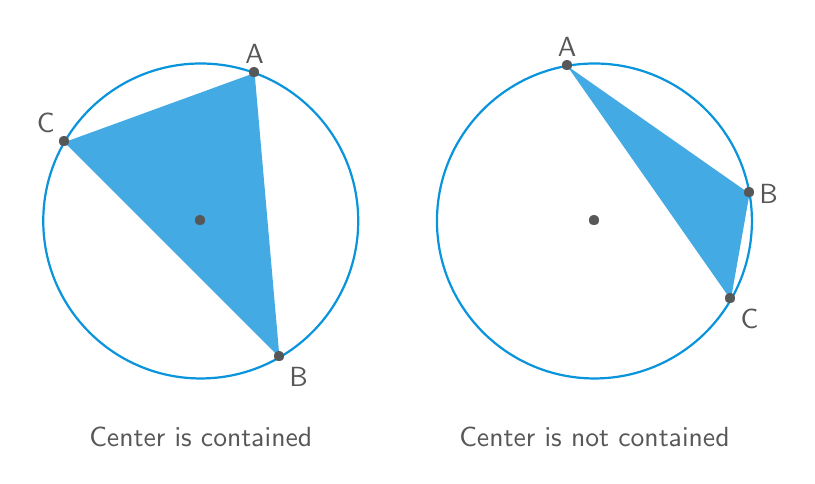
\begin{tikzpicture}
    %\draw[gray, very thin] (-3,-3) grid (3,3);
    \draw[thick,color=spot] (0,0) circle (2);
    \coordinate (A) at (70:2);
    \coordinate (B) at (-60:2);
    \coordinate (C) at (150:2);
    \path [fill=spot!75] (A) -- (B) -- (C) -- (A);
    \draw (A) node {\textbullet} node [anchor=south] {A};
    \draw (B) node {\textbullet} node [anchor=north west] {B};
    \draw (C) node {\textbullet} node [anchor=south east] {C};
    \draw (0,0) node {\textbullet};
    \draw (0, -2.5) node [anchor=north] {Center is contained};
    \draw[thick,color=spot] (0,0) +(5,0) circle (2);
    \coordinate (A) at (100:2);
    \coordinate (B) at (10:2);
    \coordinate (C) at (-30:2);
    \path [transform canvas={xshift=5cm}, fill=spot!75] (A) -- (B) -- (C) -- (A);
    \draw (A)+(5,0)  node {\textbullet} node [anchor=south] {A};
    \draw (B)+(5,0)  node {\textbullet} node [anchor=west] {B};
    \draw (C)+(5,0)  node {\textbullet} node [anchor=north west] {C};
    \draw (0,0)+(5,0)  node {\textbullet};
    \draw (5, -2.5) node [anchor=north] {Center is not contained};

\end{tikzpicture}

\end{document}